% This file was created by matlab2tikz v0.4.0.
% Copyright (c) 2008--2013, Nico Schlömer <nico.schloemer@gmail.com>
% All rights reserved.
% 
% The latest updates can be retrieved from
%   http://www.mathworks.com/matlabcentral/fileexchange/22022-matlab2tikz
% where you can also make suggestions and rate matlab2tikz.
% 
% 
% 
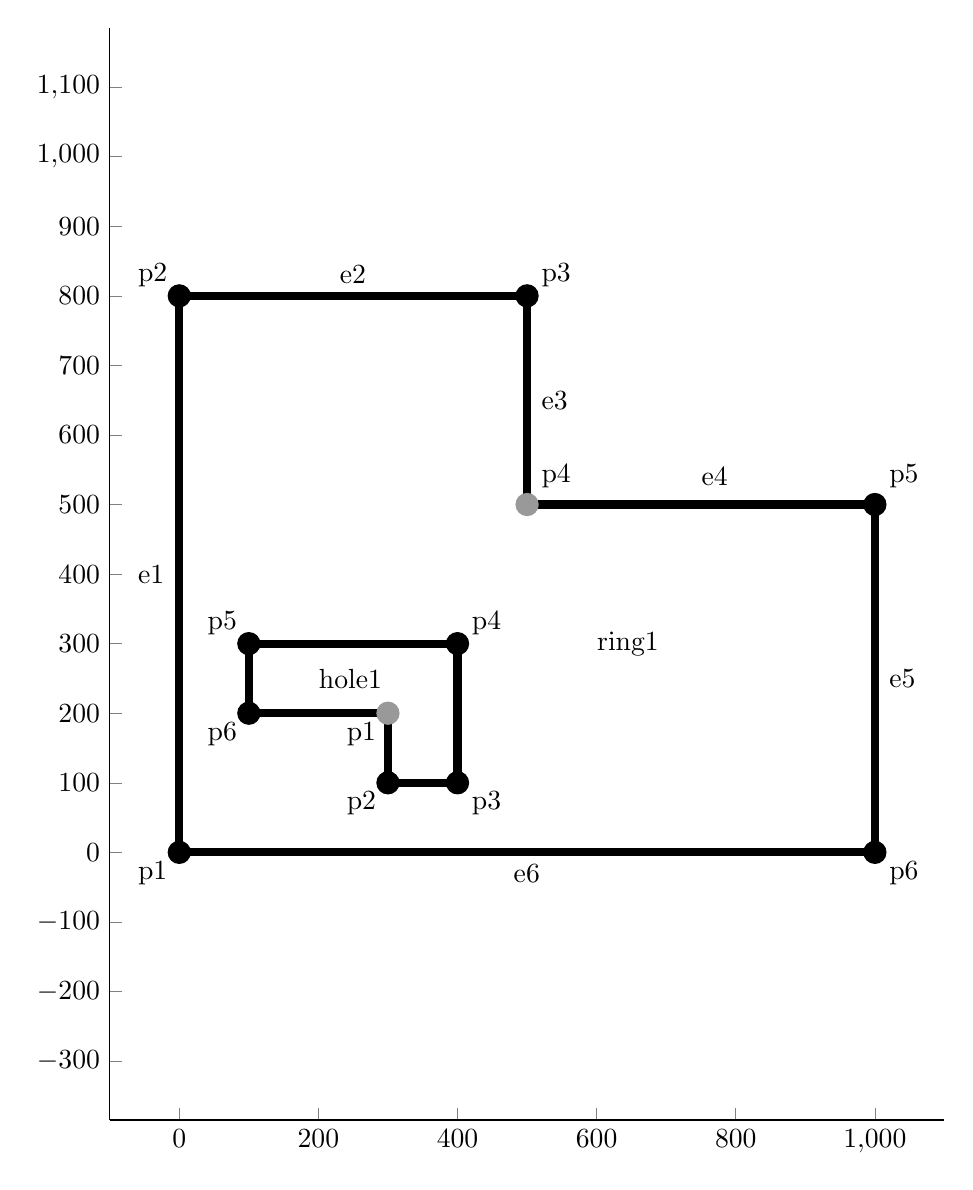
\begin{tikzpicture}

\begin{axis}[%
width=4.17369791666667in,
height=5.45880208333333in,
scale only axis,
xmin=-100,
xmax=1100,
ymin=-384.743245772758,
ymax=1184.74324577276,
axis x line*=bottom,
axis y line*=left
]
\addplot [
color=black,
solid,
line width=3.0pt,
forget plot
]
table[row sep=crcr]{
0 0\\
1000 0\\
1000 500\\
500 500\\
500 800\\
0 800\\
0 0\\
};
\addplot [
color=black,
solid,
line width=3.0pt,
forget plot
]
table[row sep=crcr]{
300 200\\
100 200\\
100 300\\
400 300\\
400 100\\
300 100\\
300 200\\
};
\addplot [
color=black,
mark size=4.0pt,
only marks,
mark=*,
mark options={solid,fill=black},
forget plot
]
table[row sep=crcr]{
0 0\\
1000 0\\
1000 500\\
500 800\\
0 800\\
};
\addplot [
color=black,
mark size=4.0pt,
only marks,
mark=*,
mark options={solid,fill=black},
forget plot
]
table[row sep=crcr]{
100 200\\
100 300\\
400 300\\
400 100\\
300 100\\
};
\addplot [
color=lightgray!80!black,
mark size=4.0pt,
only marks,
mark=*,
mark options={solid,fill=lightgray!80!black},
forget plot
]
table[row sep=crcr]{
300 200\\
};
\addplot [
color=lightgray!80!black,
mark size=4.0pt,
only marks,
mark=*,
mark options={solid,fill=lightgray!80!black},
forget plot
]
table[row sep=crcr]{
500 500\\
};
\node[right, inner sep=0mm, text=black]
at (axis cs:600,300,0) {ring1};
\node[right, inner sep=0mm, text=black]
at (axis cs:200,250,0) {hole1};
\node[right, inner sep=0mm, text=black]
at (axis cs:-60,-30,0) {p1};
\node[right, inner sep=0mm, text=black]
at (axis cs:480,-30,0) {e6};
\node[right, inner sep=0mm, text=black]
at (axis cs:-60,400,0) {e1};
\node[right, inner sep=0mm, text=black]
at (axis cs:-60,830,0) {p2};
\node[right, inner sep=0mm, text=black]
at (axis cs:520,830,0) {p3};
\node[right, inner sep=0mm, text=black]
at (axis cs:520,540,0) {p4};
\node[right, inner sep=0mm, text=black]
at (axis cs:1020,540,0) {p5};
\node[right, inner sep=0mm, text=black]
at (axis cs:1020,-30,0) {p6};
\node[right, inner sep=0mm, text=black]
at (axis cs:230,830,0) {e2};
\node[right, inner sep=0mm, text=black]
at (axis cs:520,650,0) {e3};
\node[right, inner sep=0mm, text=black]
at (axis cs:750,540,0) {e4};
\node[right, inner sep=0mm, text=black]
at (axis cs:1020,250,0) {e5};
\node[right, inner sep=0mm, text=black]
at (axis cs:240,170,0) {p1};
\node[right, inner sep=0mm, text=black]
at (axis cs:40,170,0) {p6};
\node[right, inner sep=0mm, text=black]
at (axis cs:40,330,0) {p5};
\node[right, inner sep=0mm, text=black]
at (axis cs:420,330,0) {p4};
\node[right, inner sep=0mm, text=black]
at (axis cs:420,70,0) {p3};
\node[right, inner sep=0mm, text=black]
at (axis cs:240,70,0) {p2};
\end{axis}
\end{tikzpicture}%